\section{Introduction}
\label{sec:intro}

In digital simulations of life the goal is to induce the emergence of certain
structures or processes. These might include self-replicating or autopoietic
organisms, evolutionary processes, and intelligent behavior. Often identifying
the growth of these structures and processes is reduced to identifying a growth
in complexity. Hence designers of artificial life simulations are interested in
the question of measuring complexity.

As artificial life simulations scale, quantitative assessment of the
simulation's success in meeting the designer's criteria is essential.
Identifying and selecting amongst the design choices of a given simulation in a
qualitative manner is not scalable and likely to admit experimental bias. As an
analogy, imagine constructing a machine-learning model to learn a given task
without an objective function. Curiosity driven exploration and reinforcement
learning can result in the model learning to successfully complete the task.
However, from the empiricists perspective, assessing the ability of the model
at completing the task is critical. At the very least, some criterion is needed
for evaluating the model, if not training it. Similarly, in artificial life,
while the measure of complexity is typically not used as an objective to guide
the active simulation, it is at least essential to evaluate the post-hoc
success of the simulation.

Complexity is notoriously ill-defined and difficult to measure objectively. One
of the challenges in measuring complexity is identifying the ``Goldilock's
zone'' between total order and total disorder where complexity may reside
(\emph{c.f.} figure~\ref{fig:complexity_and_entropy}). Information theoretic
measures such as Shannon entropy~\citep{shannon1948} and Kolmogorov complexity
(sometimes called Algorithmic Information Content)~\citep{kolmogorov1965,
solomonoff1964}, are actually measures of randomness. As
figure~\ref{fig:complexity_and_entropy} illustrates, these measures increase
monotonically with the disorder of a system.

\begin{figure}
\centering
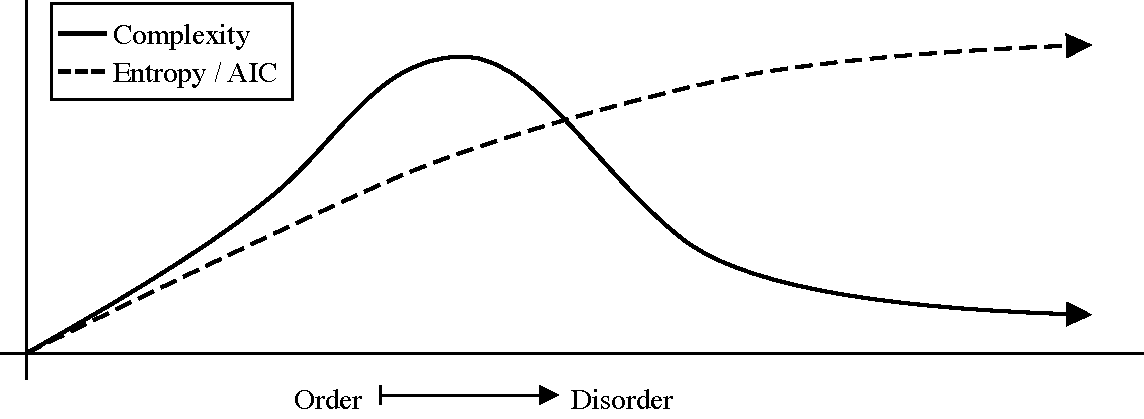
\includegraphics[width=0.7\textwidth]{figures/complexity_and_entropy}
\caption{TODO}
\label{fig:complexity_and_entropy}
\end{figure}
